% Chapter Template

\chapter{Cross section measurement} % Main chapter title

\label{Chapter7} % Change X to a consecutive number; for referencing this chapter elsewhere, use \ref{ChapterX}

\lhead{Chapter 7. \emph{Cross section measurement}} % Change X to a consecutive number; this is for the header on each page - perhaps a shortened title


Cross section for pp$\rightarrow$W+bb process is measured separately in electron and muon channel using this simple relation:
\begin{equation}
\sigma = \frac{N_{sig}}{A\times \epsilon \cdot \mathcal{L}}
\end{equation}
where $N_{sig}$ is the number of signal events after applying selection criteria described in \ref{sec:selection}, $A\times \epsilon$ is the detector acceptance and efficiency (section \ref{sec:AE}) and $\mathcal{L}$ is the total integrated luminosity for the period over the which data was collected described in \ref{sec:lumi}. 
\par In the following sections the fitting procedure for the extraction of signal events is described taking into account the systematic effects. After the subtraction of background contribution, final $N_{sig}$ for cross section calculation was obtained. The procedure for calculation of $A\times \epsilon$ is described in \ref{sec:AE}. Finally, cross section are computed and compared to theoretical predictions. 

%----------------------------------------------------------------------------------------
%	SECTION 2
%----------------------------------------------------------------------------------------

\section{Fitting procedure}

After applying selection criteria described in section \ref{sec:selection}, transverse mass distributions are obtained for both electron and muon channels. Modeling signal region was done using four-flavor scheme and five-flavor scheme separately. These samples are described in detail in \ref{sec:samples}. The comparison between the two samples is given in figure \ref{fig:4fsvs5fs}.
\begin{figure}[htbp]
	\centering
		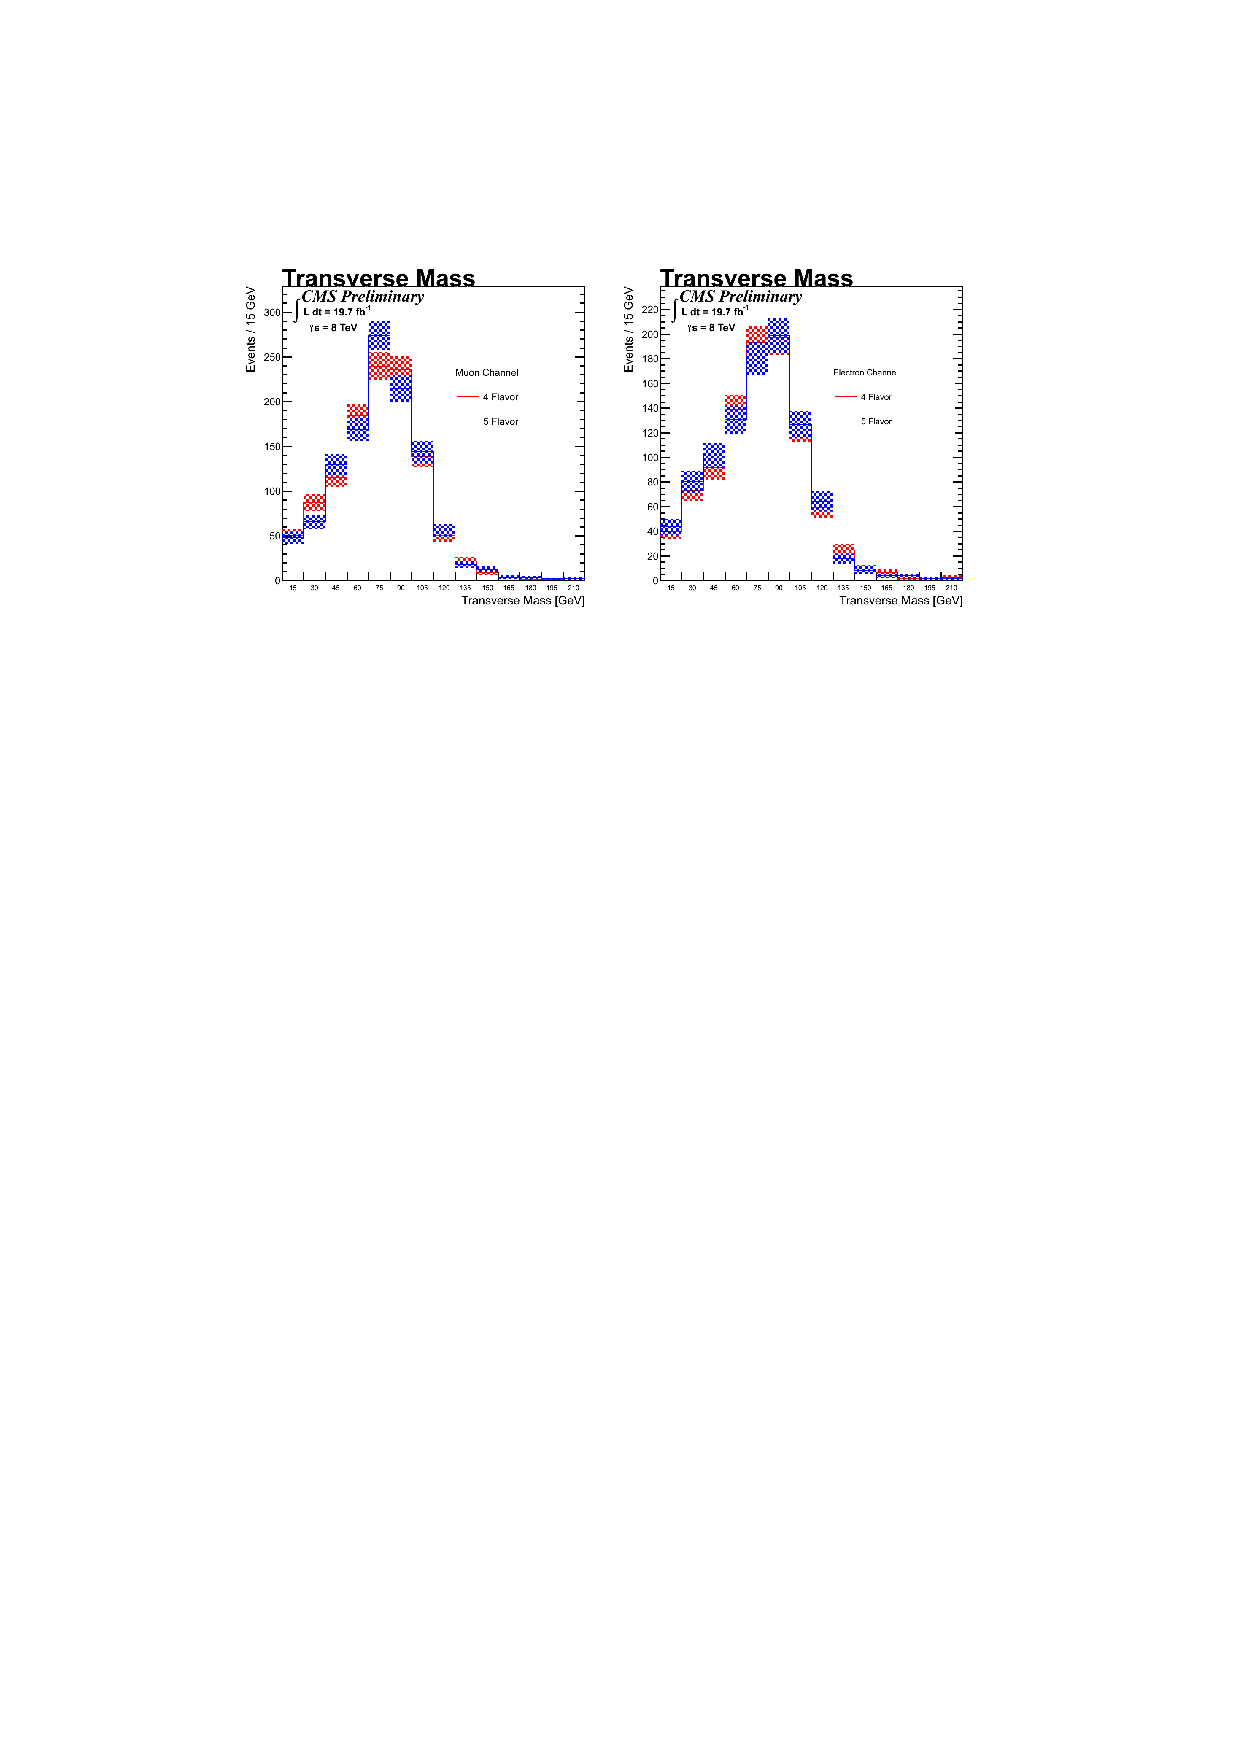
\includegraphics[width=\textwidth]{Figures/4fsvs5fs.pdf}
	\caption[Comparison of the two W+bb samples used to obtain the number of signal events.]{Shape comparison of the two samples used to obtain the number of signal events. Left figure shows muon channel while the right figure shows the electron channel.}
	\label{fig:4fsvs5fs}
\end{figure}

Final signal yields are extracted using a binned maximum likelihood fit. Simultaneous fit was performed in Wbb region and in TT multijet control region. The result of the fit is represented as \textit{signal strength} $\mu$ which is the ratio between the cross section under test and the theoretical cross section.    
For each shape uncertainty and process/channel affected by it, two additional input shapes have to be provided, obtained shifting that parameter up and down by one standard deviation. When building the likelihood, each shape uncertainty is associated to a nuisance parameter taken from a unit gaussian distribution, which is used to interpolate or extrapolate using the specified histograms.

%----------------------------------------------------------------------------------------
%	SECTION 3
%----------------------------------------------------------------------------------------

\section{Systematics}

Systematic uncertainties on the expected signal and background yields and shapes affect
the final distribution used to obtain $N_{sig}$. For a given systematic variation, a new set of signal and background templates was created which may differ both in shape and normalization from the original template.  These shape variations are included in the final fit. Several sources of systematic variations have been considered:

\begin{itemize}
        \item{\textbf{Luminosity:}}
        an uncertainty of 2.2\% for luminosity measurement during 2012 datataking is reported by the CMS luminosity group.
        \item{\textbf{Jet energy scale:}}
        the jet energy scale for each jet is varied within one standard deviation of the applied jet energy corrections based on $p_T$ and $\eta$ of the jet, and the efficiency of the analysis selection is recomputed to assess the systematic variation on the normalization and shape of the signal and all background components.
        \item{\textbf{Jet energy resolution:}}
        jet energy resolution in simulation is smeared by default in order to take into account worse resolution in data. The uncertainty on the applied smearing factors is used to produce modified signal and background templates are created and used in the final fit.
        \item{\textbf{Lepton energy scale:}}
        muon and electron trigger, reconstruction, and identification efficiencies are determined in data using the standard tag-and-probe technique with Z bosons. The systematic uncertainty is evaluated by varying lepton energy scale for each lepton type within one standard deviation taken from POG.
        \item{\textbf{Unclustered missing energy:}}
        we follow the suggested procedure from the JetMET POG to determine the systematic uncertainty on the calibration of unclustered MET (missing energy associated with particles not clustered into jets).
        \item{\textbf{MC samples normalizations:}}
        the finite size of the signal and background MC samples are included in the normalization uncertainties. Normalizations for each of the Monte-Carlo samples are also allowed to vary within the uncertainties of measured Standard model cross-sections. Cross section uncertainties are summarized in the table \ref{tab:SMunc}
        \item{\textbf{Jet b-tagging:}}
        official b-tagging scale factors are applied consistently to jets in signal and background events.
\end{itemize}

\begin{table}[!htb]
\begin{center}
   \begin{tabular} {r c} \hline \hline
        Process         & Cross section uncertainty \\
        \hline
        W+c(c)          & 8.1$\%$ \\
        W+udsg          & 13.2$\%$ \\
        Z+jets          & 7.9$\%$ \\
        Single Top      & 5.4$\%$ \\
        T$\bar{T}$      & 7.4$\%$ \\
        VV              & 8.1$\%$ \\
        \hline\hline
   \end{tabular}
\caption{Standard model cross section uncertainties used in the evaluation of MC normalization systematic effect.}
\label{tab:SMunc}
\end{center}
\end{table}

Shape variations used in the final fit are shown in the figure \ref{fig:shapeVar}. Contributions from different sources of systematic variations are summarized in Table \ref{tab:systContrib}. Table also shows relative contribution to the signal strength uncertainty for each source of uncertainty together with the change in total systematic uncertainty when removing specific source of uncertainty.

\begin{figure}[htbp]
	\centering
		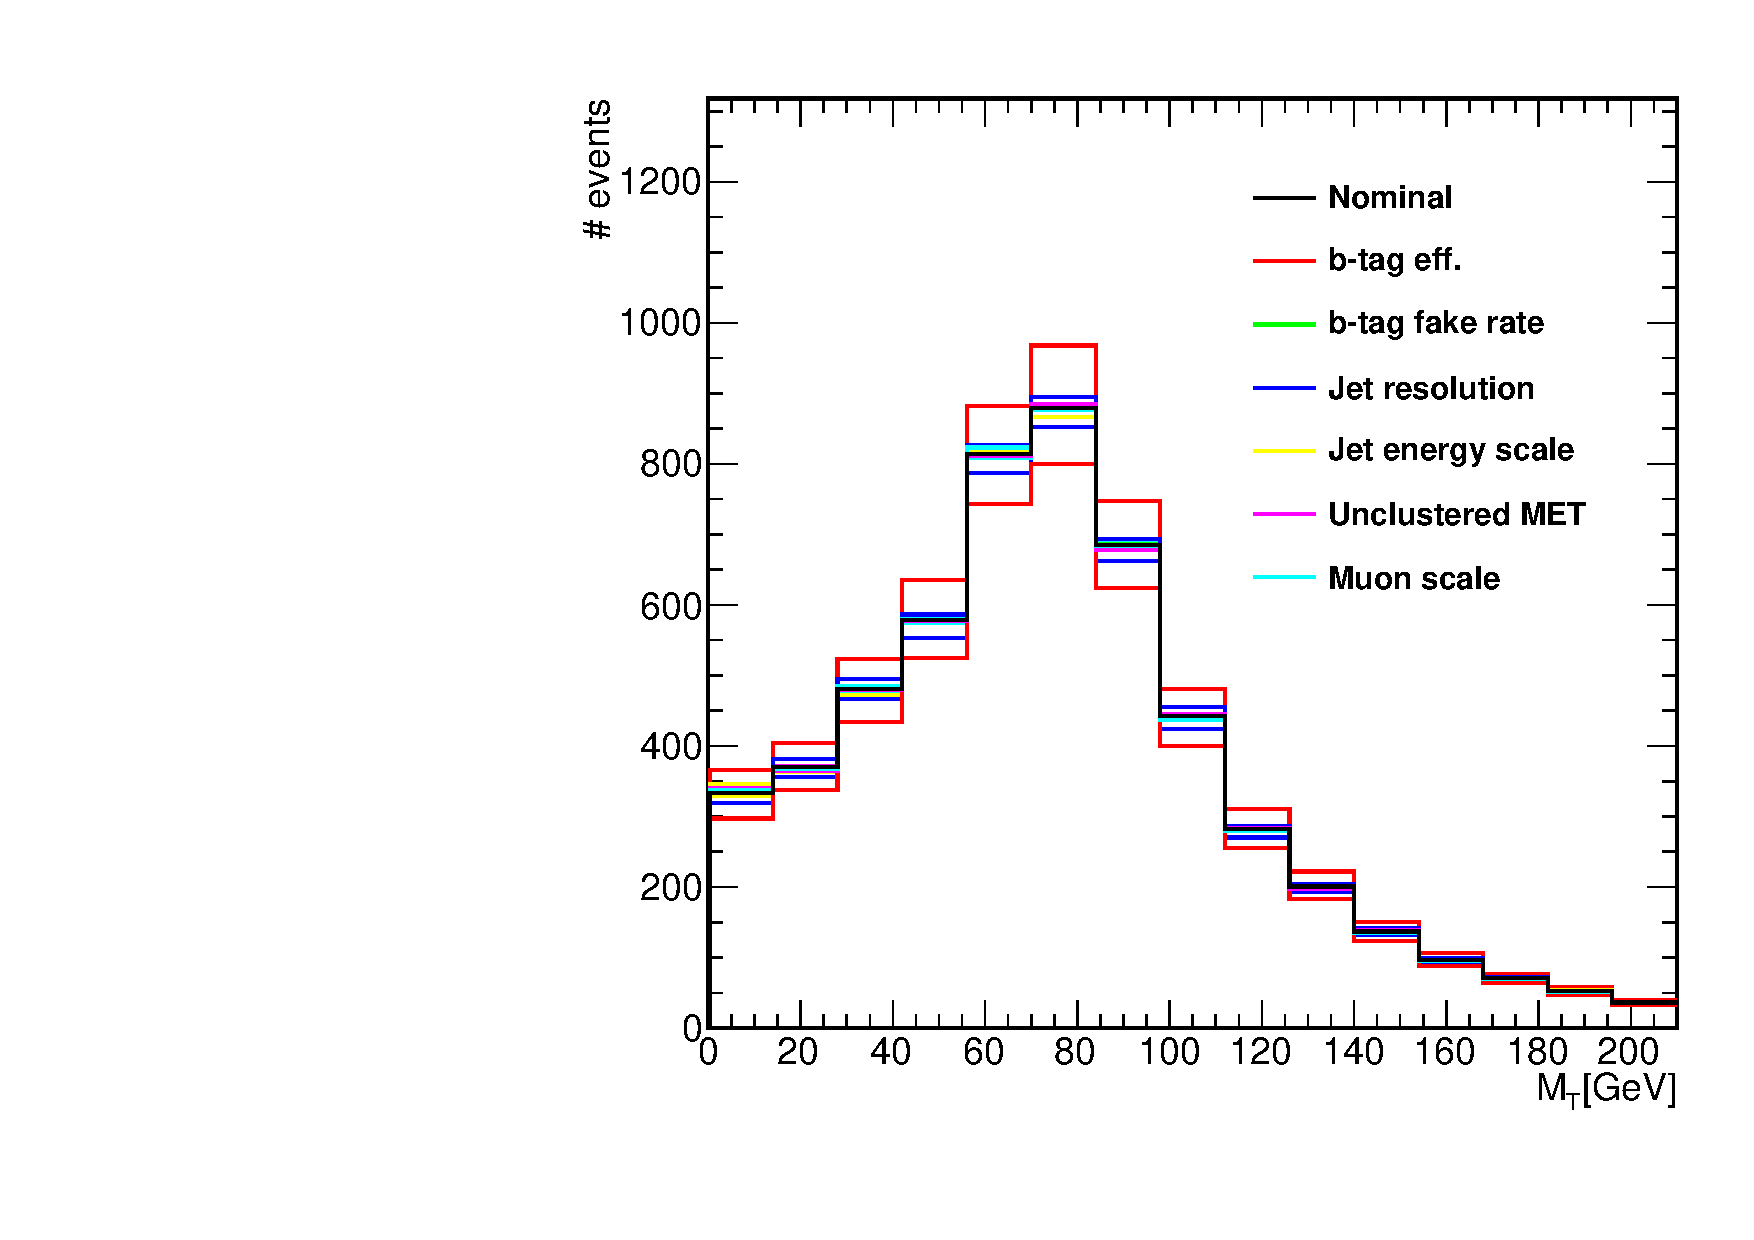
\includegraphics[width=0.49\textwidth]{Figures/syst_Wbb_var.pdf}
		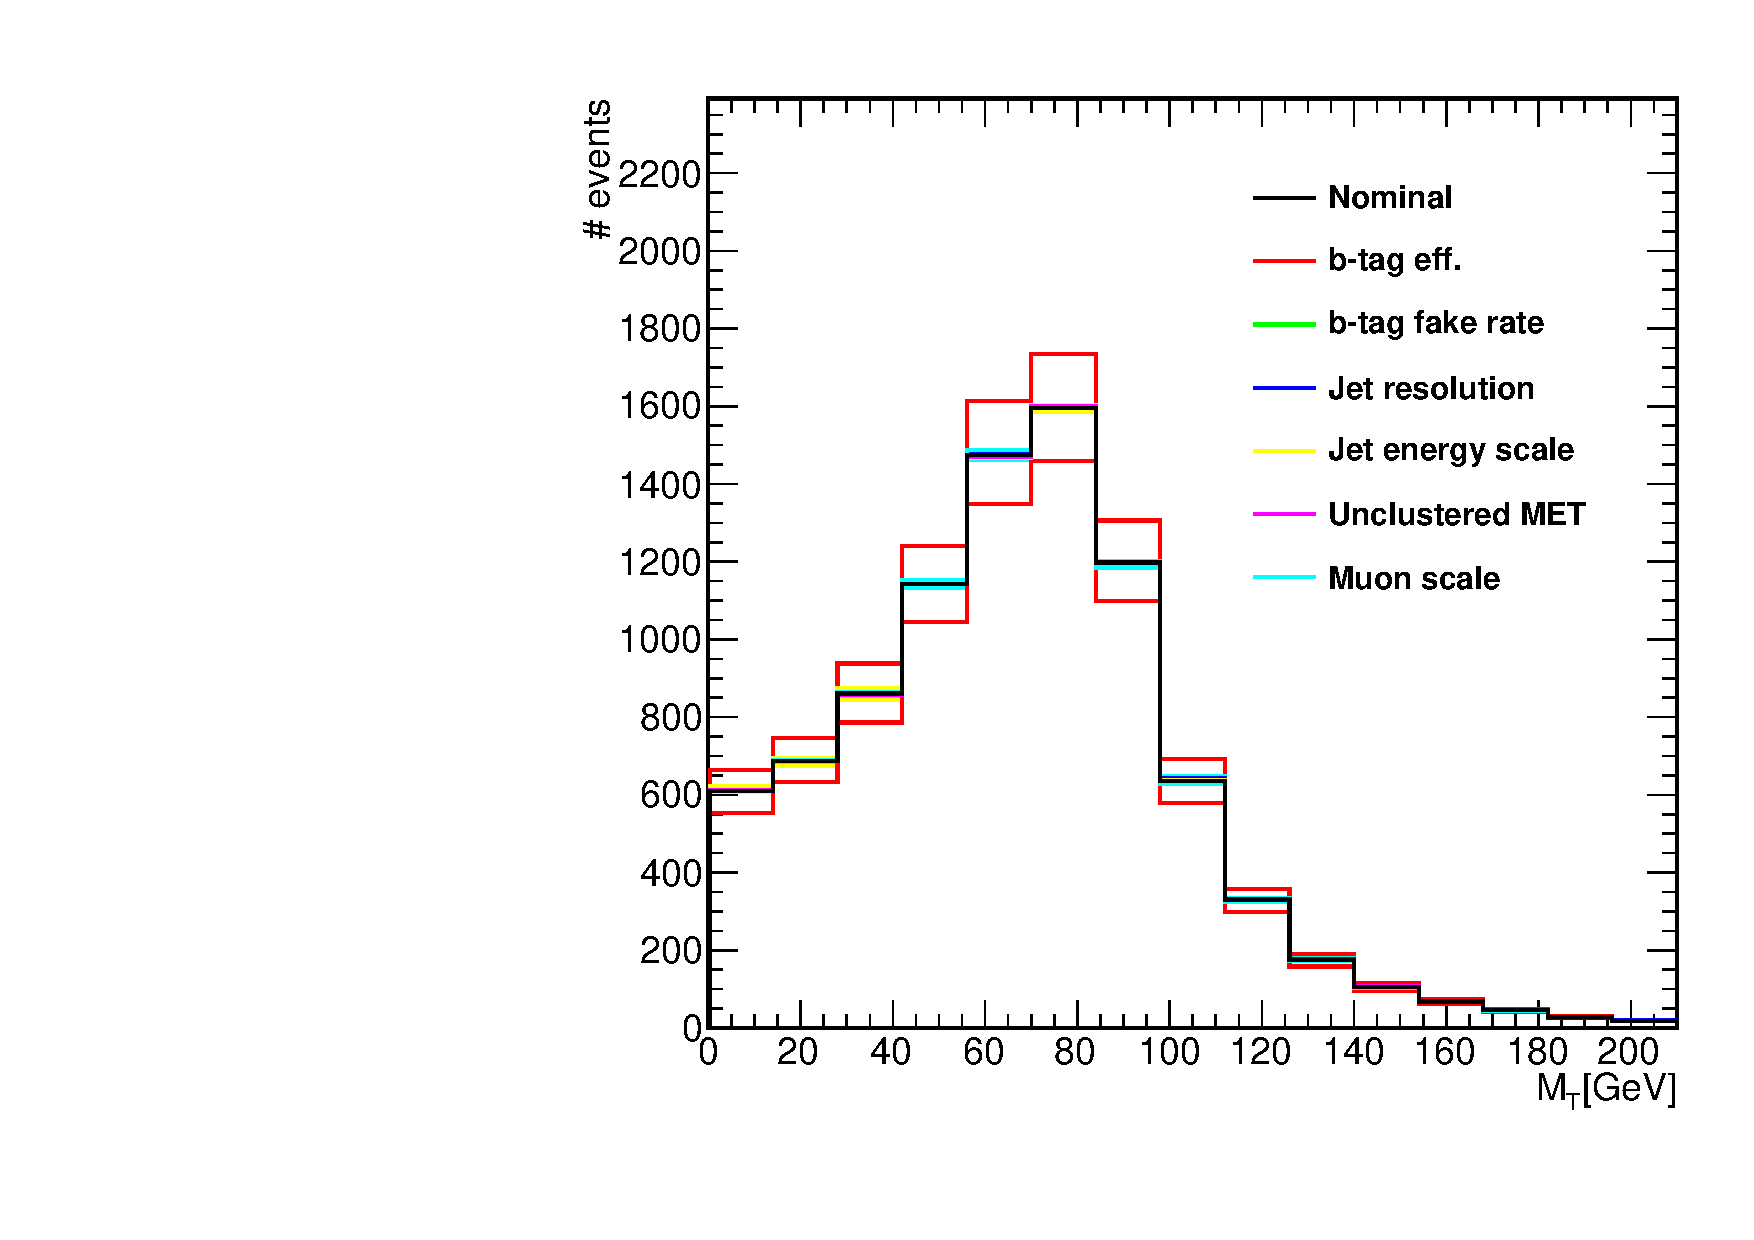
\includegraphics[width=0.49\textwidth]{Figures/syst_TT_var.pdf}
	\caption[Shape of the transverse mass distribution for each systematic variation in both, signal region and TT control region.]{Shape of the transverse mass distribution in the muon channel for each systematic variation in both, signal region (left) and TT control region(right).}
	\label{fig:shapeVar}
\end{figure}

%----------------------------------------------------------------------------------------
%	SECTION 3
%----------------------------------------------------------------------------------------

\section{Acceptance and efficiency}
\label{sec:AE}
    
Due to the limitations of the detector, not all produced signal events will be detected. Some final state particles will end up outside the functional part of the detector. The fraction of the phase space covered with functional detector for signal final state particles is called \textit{acceptance}. Usually this part of the phase space is called \textit{fiducial region} and applied cuts are summarized in table \ref{tab:fiducial}.             
\begin{table}[!htb]
\begin{center}
   \begin{tabular} {l l} \hline \hline
        Variable         & Cut \\
        \hline
        Lepton $p_T$    & $>$ 30\ GeV \\
        Lepton $|\eta|$   & $<$ 2.1 \\
        Jet $p_T$       & $>$ 25  \\
        Jet $|\eta|$      & $<$ 2.4 \\
        \multicolumn{2}{l}{
        Jet matched to a B hadron within a cone of 0.5} \\
        \hline\hline
   \end{tabular}
\caption{Fiducial cuts used for cross section measurements.}
\label{tab:fiducial}
\end{center}
\end{table}
However, fraction of the events that fall into the fiducial volume will not be detected due to trigger and reconstruction inefficiency or selection cuts imposed by trigger or the analysis. Usually, acceptance and efficiency are estimated as a single quantity which is a product of these two numbers, defined as:
\begin{equation}
A\times \epsilon=\frac{\mathrm{number\ of\ selected\ Wbb\ events}}{\mathrm{number\ of\ generated\ Wbb\ events\ in\ the\ fiducial\ volume}}
\end{equation}
This ratio is computed using simulated Wbb sample for each of the channels separately. Number of selected events is obtained by applying the selection cuts described in \ref{sec:selection}. Number of generated hits is obtained by applying generator-level cuts summarized in the table \ref{tab:fiducial}. With this ratio being derived from simulation, it is necessary to correct it for the difference between data and Monte-Carlo. These corrections include pile-up  $w^{PU}$, lepton trigger, reconstruction and identification scale factors $w^{lep}$, and b-tagging scale factors $w^{b-tag}$ all described in \ref{sec:mcSF}. With all the corrections, $A\times \epsilon$ for each channel becomes:
\begin{equation}
A\times \epsilon = \frac{\sum^{sel} w^{lep} w^{PU} w^{b-tag}}{N_{fiducial}^{gen}}
\end{equation}

Obtained results are summarized in the table \ref{tab:AE} for each channel.

\begin{table}[!htb]
\begin{center}
   \begin{tabular} {r c} \hline \hline
        Channel         & A$\times \epsilon$ \\
        \hline
        Muon channel         & 8.1$\%$ \\
        Electron channel     & 7.8$\%$ \\
        \hline\hline
   \end{tabular}
\caption{Results of the A$\times \epsilon$ measurement for both, muon and electron channel.}
\label{tab:AE}
\end{center}
\end{table}



%----------------------------------------------------------------------------------------
%	SECTION 5
%----------------------------------------------------------------------------------------

\section{Results}
\label{sec:res}

\subsection{Double parton scattering contribution}

%
%\begin{table}[!htb]
%\begin{center}
%\begin{tabular}{ccccc} \hline \hline
%&  & Event yield uncertainty &Individual contribution & Effect of removal  \\
%Source & Type & range (\%) &  to $\mu$ uncertainty (\%) & on $\mu$ uncertainty (\%) \\ \hline
%b-tag efficiency & shape &
%10.34 & 1.48 & 1.73\\
%b-tag fake rate & shape &
%0.08 & 0.01 & 0.40\\
%Jet resolution & shape &
%0.01 & 0.02 & 0.52\\
%Jet energy scale & shape &
%0.07 & $<0.01$ & 1.36\\
%Unclustered MET & shape &
%$<0.01$ & $<0.01$ & 5.20\\
%Muon scale & shape &
%0.12 & $<0.01$ & 0.38\\
%Luminosity & norm. &
%2.60 & 1.90 & 1.21\\
%Monte Carlo statistics & norm. &
%0.78 & 2.40 & 5.83\\
%\hline
%\end{tabular}
%\caption{Information about each source of systematic uncertainty together with the information whether just normalization or shape is included in the final fit. The table also shows the uncertainty on signal and background yields and the relative contribution to the signal strength uncertainty. Due to correlations, the total systematic uncertainty is smaller that the quadrature sume of individual uncertainties. The last column shows the decreade in total systematic uncertainty when removing specific source of uncertainty.}
%\label{tab:systZG}
%\end{center}
%\end{table}
%\subsection{Fit Results \label{sec:FitZagreb}}
%
%Binned maximum likelihood fits are peformed using
%templates derived from simulation. Systematic uncertainties on the fitted scale factors are de-
%determined by evaluating the effect on the template shapes from various sources of systematics,
%including b-tagging and jet energy scale and resolution.
%Final fit is performed simultaneously fitting transverse mass distributions in both signal
%region and $t\bar{t}$ multijet control region .
%
%Final yields are summarized in the Tables \ref{tab:fitYieldsJelena} for signal region and \ref{tab:fitYieldsJelenaTT} for $t\bar{t}$ multijet control region.
%Obtained yields are found to be in a good agreement with data. Measured signal strength for Wbb of $r = 1.34 \pm 0.16$ is in good agreement with signal strengths from Results section.
%
%\begin{table}[!htb]
%\begin{center}
%   \begin{tabular} {r|l|l} \hline \hline
%\bf{W+bb} & \multicolumn{2}{c}{Fit Result: r = 1.15 $\pm$ 0.16}\\
%        Sample          & Prefit                & Postfit \\
%        \hline
%        W+bb            &370.8$\pm$12.3 &556.6\\
%        W+cc            &20.3$\pm$5.3   &24.0\\
%        W+udscg         &1.7$\pm$1.0    &1.7\\
%        Z+jets          &21.8$\pm$6.9   &22.9\\
%        Single Top      &540.7$\pm$14.2 &624.5\\
%        T$\bar{T}$      &5577.3$\pm$20.5&6383.7\\
%        VV              &25.3$\pm$1.3   &28.2\\
%        QCD             &234.4$\pm$10.7 &158.7\\
%        \hline
%        Sum             &6792.4$\pm$31.1&7906.3\\
%        \hline
%        Data&\multicolumn{2}{c}{7995.0$\pm$89.4}\\
%        \hline\hline
%   \end{tabular}
%\caption{Data and MC yields before and after the fit in $t\bar{t}$ control region.}
%\label{tab:fitYieldsJelenaTT}
%\end{center}
%\end{table}
%
%\begin{table}[!htb]
%\begin{center}
%   \begin{tabular} {r|l|l} \hline \hline
%\bf{W+bb} & \multicolumn{2}{c}{Fit Result: r = 1.34 $\pm$ 0.16}\\
%        Sample          & Prefit                & Postfit \\
%        \hline
%        W+bb            &879.7$\pm$23.2         &1350.0\\
%        W+cc            &35.5$\pm$8.2           &42.5\\
%        W+udscg         &19.7$\pm$6.9           &20.1\\
%        Z+jets          &122.5$\pm$17.3         &131.2\\
%        Single Top      &722.1$\pm$15.5         &833.0\\
%        T$\bar{T}$      &2338.6$\pm$11.1        &2676.7\\
%        VV              &106.4$\pm$2.6          &121.4\\
%        QCD             &249.3$\pm$14.9         &220.6\\
%        \hline
%        Total MC        &4473.9$\pm$39.4        &5426.1\\
%        \hline
%        Data&\multicolumn{2}{c}{5355.0$\pm$73.2}\\
%   \hline\hline
%   \end{tabular}
%\caption{Yields of MC samples before and after the fit.}
%\label{tab:fitYieldsJelena}
%\end{center}
%\end{table}
%
%
%
%
%
%\subsection{Tests of the fit stability}
%
%Additional tests were performed in order to verify the fit stability od the signal strength.
%This was done by fitting different combinations of distributions in both signal region and $t\bar{t}$ control region.
%Additional distributions include missing energy in the signal region and $t\bar{t}$ control region and
%invariant mass of third and fourth jet in $t\bar{t}$ control region. All distributions show good agreement
%in shapes between data and Monte Carlo. Fitting procedure is the as described in section \ref{sec:FitZagreb}.
%Obtained signal strengths are summarized in Table \ref{tab:addFitTest}.
%
%\begin{table}[!htb]
%\begin{center}
%   \begin{tabular} {ccc} \hline\hline
%   Fitted distribution (Wbb/TT) & ~~~Signal Strength~~~ & ~~~~Yield Ratio~~~ \\
%        \hline
%        $M_T$/$M_T$                     &1.34$\pm$0.15  &1.55\\
%        $M_T$/$E^{miss}_T$              &1.31$\pm$0.14  &1.52\\
%        $M_T$/$M(j_3j_4)$               &1.35$\pm$0.16  &1.53\\
%        $E^{miss}_T$/$M_T$              &1.43$\pm$0.21  &1.64\\
%        $E^{miss}_T$/$E^{miss}_T$       &1.33$\pm$0.17  &1.53\\
%        $E^{miss}_T$/$M(j_3j_4)$        &1.38$\pm$0.21  &1.55\\
%   \hline\hline
%   \end{tabular}
%                                                                                                                                                                                                 \caption{Signal strengths obtained by fitting different distributions. Signal strengths are found to be consistent with each other.}
%\label{tab:addFitTest}
%\end{center}
%\end{table}